\section{Implementation}

The paper aims to build a neural network for recognizing and classifying names from text data. For this, Python was used along with TensorFlow framework. Glove was introduced to boost performance. This unsupervised network created by standford, trains and creates links between words. Glove is very easy to use for training new data, such as rendering of words in other languages. In my case, there was enough standard data already trained by Standford. 

TensorBoard is another tool used to see the loss and how the graph (neural network) looks like.

\subsection{Why python?}

Python is an interpreted, object-oriented, high-level programming language with dynamic semantics. Its high-level built in data structures, combined with dynamic typing and dynamic binding, make it very attractive for Rapid Application Development, as well as for use as a scripting or glue language to connect existing components together. Python's simple, easy to learn syntax emphasizes readability and therefore reduces the cost of program maintenance. Python supports modules and packages, which encourages program modularity and code reuse. The Python interpreter and the extensive standard library are available in source or binary form without charge for all major platforms, and can be freely distributed.

Often, programmers fall in love with Python because of the increased productivity it provides. Since there is no compilation step, the edit-test-debug cycle is incredibly fast. Debugging Python programs is easy: a bug or bad input will never cause a segmentation fault. Instead, when the interpreter discovers an error, it raises an exception. When the program doesn't catch the exception, the interpreter prints a stack trace. A source level debugger allows inspection of local and global variables, evaluation of arbitrary expressions, setting breakpoints, stepping through the code a line at a time, and so on. The debugger is written in Python itself, testifying to Python's introspective power. On the other hand, often to add a few print statements to the source is the quickest way to debug a program: the fast edit-test-debug cycle makes this simple approach very effective.

Python language is one of the most flexible languages. It can be used for various purposes. Python has gained huge popularity base of this. Python does contain special libraries for machine learning namely scipy and numpy which great for linear algebra and getting to know kernel methods of machine learning. When want to work with machine learning algorithms python is great to use. It has easy syntax relatively. For beginners, this is the best language to use and to start with.

Whether a startup or an MNC, Python provides a huge list of benefits to all. The usage of Python is such that it cannot be limited to only one activity. Its growing popularity has allowed it to enter into some of the most popular and complex processes like Artificial Intelligence (AI), Machine Learning (ML), natural language processing, data science etc. The question is why Python is gaining such momentum in AI? And the answer lies below:

\begin{itemize}
    \item Less Code: AI involves algorithms - a LOT of them. Python provides ease of testing -  one of the best among competitors. Python helps in easy writing and execution of codes. Python can implement the same logic with as much as 1/5th code as compared to other OOPs languages. Thanks to its interpreted approach which enables check as you code methodology.
    \item Prebuilt Libraries: Python has a lot of libraries for every need of your AI project. Few names include Scipy for advanced computing, Numpy for scientific computation and Pybrain for machine learning. AIMA - is a library implemented in Python of algorithms from Russell and Norvig's 'Artificial Intelligence: A Modern Approach' is one of the best library available for Artificial Intelligence till today. Such a dedicated library saves developer’s time spent on coding base level items.
    \item Support: Python is a completely open source with a great community. There is a host of resources available which can get any developer up to speed in no time. There is a huge community of active coders willing to help programmers in every stage of developing cycle.
    \item Platform Agnostic: Python provides the flexibility to provide an API from an existing language which indeed provides extreme flexibility. It is also platform independent. With just a few changes in codes, you can get your app up and running in a new OS. This saves developers time in testing on different platforms and migrating code.
    \item Flexibility: Flexibility is one of the core advantages of Python. Python is suitable for every purpose with the option to choose between OOPs approach and scripting. It works as a perfect backend and it also suitable for linking different data structures together. A big plus for developers who are struggling between different algorithms is the option to check a majority of code in the IDE itself.
    \item Popularity: Python is winning the heart of millennials. It's ease of learning. Though AI Projects need a highly experienced programmer yet Python can smoothen the learning curve. It is practically more easy to look for Python developers than to hunt for LISP or Prolog programmers, particularly in some nations. Its extended libraries and active community with an ever developing and improving code have led it to be one of the hottest languages today.
\end{itemize}

Python is simple, elegant, consistent, and math-like.
\subsection{Tensor flow}

TensorFlow is an open source software library for high performance numerical computation. Its flexible architecture allows easy deployment of computation across a variety of platforms (CPUs, GPUs, TPUs), and from desktops to clusters of servers to mobile and edge devices. Originally developed by researchers and engineers from the Google Brain team within Google’s AI organization, it comes with strong support for machine learning and deep learning and the flexible numerical computation core is used across many other scientific domains.

Everything in TensorFlow is based on creating a computational graph. Think of a computational graph as a network of nodes, with each node known as an operation, running some function that can be as simple as addition or subtraction to as complex as some multi variate equation.

An Operation also referred to as op can return zero or more tensors which can be used later on in the graph. Heres a list of operations with their output for example.

Each operation can be handed a constant, array, matrix or n-dimensional matrix. Another word for an n-dimensional matrix is a tensor, a 2-dimensional tensor is equivalent to a m x m matrix.

\begin{figure}[H]
    \centering
    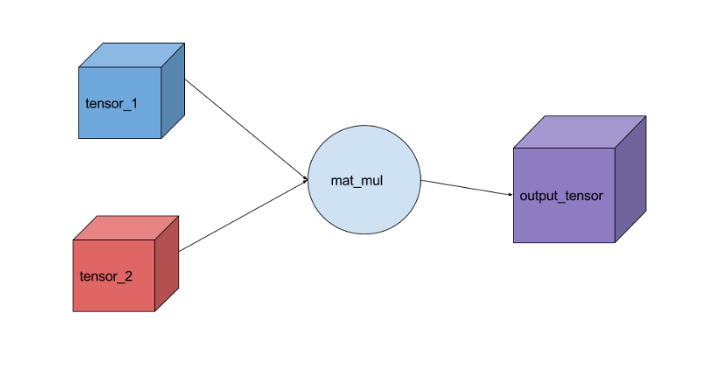
\includegraphics[width=6.5in]{images/tensor.png}
    \caption{Trivial tensor example.}
\end{figure}

The code above is creating two constant tensors and multiplying them together and outputting our result. This is a trivial example that demonstrates how you can create a graph and run the session. All inputs needed by the op are run automatically. They’re typically ran in parallel. This session run actually causes the execution of three operations in the graph, creating the two constants then the matrix multiplication.

\subsubsection{Graph}

The constants and operation was automagically added to the graph in TensorFlow. The graph default is instantiated when the library is imported. Creating a Graph object instead of using the default graph is useful when creating multiple models in one file that do not depend on each other.

\begin{lstlisting}[language=Python]
    new_graph = tf.Graph()
    with new_graph.as_default():
        new_g_const = tf.constant([1., 2., 3.])
\end{lstlisting}

any variables or operations used outside of the "with new\_graph.as\_default()" will be added to the default graph that is created when the library is loaded. You can even get a handle to the default graph with

\begin{lstlisting}[language=Python]
    default_g = tf.get_default_graph()
\end{lstlisting}

for most cases it’s best to stick with the default graph.

\subsubsection{Session}

This encapsulates the environment that operations and tensors are executed and evaluated. Sessions can have their own variables, queues and readers that are allocated. So it’s important to use the close() method when the session is over. There are 3 arguments for a Session, all of which are optional.

\begin{itemize}
    \item target: (Optional.) The execution engine to connect to. Defaults to using an in-process engine. 
    \item graph: (Optional.) The Graph to be launched. If no graph argument is specified when constructing the session, the default graph will be launched in the session. If you are using more than one graph (created with tf.Graph() in the same process, you will have to use different sessions for each graph, but each graph can be used in multiple sessions. In this case, it is often clearer to pass the graph to be launched explicitly to the session constructor.
    \item config: (Optional.) A ConfigProto protocol buffer with configuration options for the session.
\end{itemize}

\subsubsection{Placeholder}

As mentioned before, it all starts with placeholders. We need two placeholders in order to fit our model: X contains the network's inputs (the stock prices of all S\&P 500 constituents at time T = t) and Y the network's outputs (the index value of the S\&P 500 at time T = t + 1).

The shape of the placeholders correspond to [None, n\_stocks] with [None] meaning that the inputs are a 2-dimensional matrix and the outputs are a 1-dimensional vector. It is crucial to understand which input and output dimensions the neural net needs in order to design it properly.

\begin{lstlisting}[language=Python]
    # Placeholder
    X = tf.placeholder(dtype=tf.float32, shape=[None, n_stocks])
    Y = tf.placeholder(dtype=tf.float32, shape=[None])
\end{lstlisting}

The None argument indicates that at this point we do not yet know the number of observations that flow through the neural net graph in each batch, so we keep if flexible. We will later define the variable batch\_size that controls the number of observations per training batch.

\subsubsection{Variable}

Besides placeholders, variables are another cornerstone of the TensorFlow universe. While placeholders are used to store input and target data in the graph, variables are used as flexible containers within the graph that are allowed to change during graph execution. Weights and biases are represented as variables in order to adapt during training. Variables need to be initialized, prior to model training. We will get into that a litte later in more detail.

The model consists of four hidden layers. The first layer contains 1024 neurons, slightly more than double the size of the inputs. Subsequent hidden layers are always half the size of the previous layer, which means 512, 256 and finally 128 neurons. A reduction of the number of neurons for each subsequent layer compresses the information the network identifies in the previous layers. Of course, other network architectures and neuron configurations are possible but are out of scope for this introduction level article.

\begin{lstlisting}[language=Python]
    # Model architecture parameters
    n_stocks = 500
    n_neurons_1 = 1024
    n_neurons_2 = 512
    n_neurons_3 = 256
    n_neurons_4 = 128
    n_target = 1
    # Layer 1: Variables for hidden weights and biases
    W_hidden_1 = tf.Variable(
            weight_initializer(
                [n_stocks, n_neurons_1]))
    bias_hidden_1 = tf.Variable(
            bias_initializer(
                [n_neurons_1]))
    # Layer 2: Variables for hidden weights and biases
    W_hidden_2 = tf.Variable(
            weight_initializer(
                [n_neurons_1, n_neurons_2]))
    bias_hidden_2 = tf.Variable(
            bias_initializer(
                [n_neurons_2]))
    # Layer 3: Variables for hidden weights and biases
    W_hidden_3 = tf.Variable(
            weight_initializer(
                [n_neurons_2, n_neurons_3]))
    bias_hidden_3 = tf.Variable(
            bias_initializer(
                [n_neurons_3]))
    # Layer 4: Variables for hidden weights and biases
    W_hidden_4 = tf.Variable(
            weight_initializer(
                [n_neurons_3, n_neurons_4]))
    bias_hidden_4 = tf.Variable(
            bias_initializer(
                [n_neurons_4]))
    
    # Output layer: Variables for output weights and biases
    W_out = tf.Variable(
            weight_initializer(
                [n_neurons_4, n_target]))
    bias_out = tf.Variable(
            bias_initializer(
                [n_target]))
\end{lstlisting}

It is important to understand the required variable dimensions between input, hidden and output layers. As a rule of thumb in multilayer perceptrons (MLPs, the type of networks used here), the second dimension of the previous layer is the first dimension in the current layer for weight matrices. This might sound complicated but is essentially just each layer passing its output as input to the next layer. The biases dimension equals the second dimension of the current layer’s weight matrix, which corresponds the number of neurons in this layer.

\subsubsection{Scope}

Variables and tensors in TensorFlow have a name attribute that is used to identify them in the symbolic graph. If you don't specify a name when creating a variable or a tensor, TensorFlow automatically assigns a name for you:

\begin{lstlisting}[language=Python]
    a = tf.constant(1)
    print(a.name)  # prints "Const:0"
    
    b = tf.Variable(1)
    print(b.name)  # prints "Variable:0"
\end{lstlisting}

You can overwrite the default name by explicitly specifying it:

\begin{lstlisting}[language=Python]
    a = tf.constant(1, name="a")
    print(a.name)  # prints "a:0"
    
    b = tf.Variable(1, name="b")
    print(b.name)  # prints "b:0"
\end{lstlisting}

TensorFlow introduces two different context managers to alter the name of tensors and variables. The first is tf.name\_scope:

\begin{lstlisting}[language=Python]
    with tf.name_scope("scope"):
    a = tf.constant(1, name="a")
    print(a.name)  # prints "scope/a:0"
    
    b = tf.Variable(1, name="b")
    print(b.name)  # prints "scope/b:0"
    
    c = tf.get_variable(name="c", shape=[])
    print(c.name)  # prints "c:0"
\end{lstlisting}

Note that there are two ways to define new variables in TensorFlow, by creating a tf.Variable object or by calling tf.get\_variable. Calling tf.get\_variable with a new name results in creating a new variable, but if a variable with the same name exists it will raise a ValueError exception, telling us that re-declaring a variable is not allowed.

tf.name\_scope affects the name of tensors and variables created with tf.Variable, but doesn't impact the variables created with tf.get\_variable.

Unlike tf.name\_scope, tf.variable\_scope modifies the name of variables created with tf.get\_variable as well:

\begin{lstlisting}[language=Python]
    with tf.variable_scope("scope"):
        a = tf.constant(1, name="a")
        print(a.name)  # prints "scope/a:0"
        
        b = tf.Variable(1, name="b")
        print(b.name)  # prints "scope/b:0"
        
        c = tf.get_variable(name="c", shape=[])
        print(c.name)  # prints "scope/c:0"
  
    with tf.variable_scope("scope"):
        a1 = tf.get_variable(name="a", shape=[])
        a2 = tf.get_variable(name="a", shape=[])  # Disallowed
\end{lstlisting}

But what if we actually want to reuse a previously declared variable? Variable scopes also provide the functionality to do that:

\begin{lstlisting}[language=Python]
    with tf.variable_scope("scope"):
        a1 = tf.get_variable(name="a", shape=[])
    with tf.variable_scope("scope", reuse=True):
        a2 = tf.get_variable(name="a", shape=[])  # OK
\end{lstlisting}

\subsubsection{Loss}

Loss is the target function that the optimization algorithm will try to minimize.

In general, you want your loss function to be a measure of how bad your model is. But because the optimization algorithms require a few mathematical properties to work nicely, you can't pick the usual stuff like precision and recall (you want continuous functions that are differentiable in relation to the model parameters).

With classification tasks, softmax is a common choice. It's a smooth and well-behaved version of argmax, which is used to pick the class with highest network activation. With regression, the usual mean squared error serves fine.

\subsubsection{Logits}

Logit is a function. This will map probabilities [0, 1] to [-inf, +inf].

Softmax is a function that maps [-inf, +inf] to [0, 1] similar as Sigmoid. But Softmax also normalizes the sum of the values(output vector) to be 1.

Tensorflow "with logit": It means that you are applying a softmax function to logit numbers to normalize it. The input\_vector/logit is not normalized and can scale from [-inf, inf].

For multiclass classification problems is used this normalization. And sigmoid normalization is used for multilabel classification problems i.e. 
\begin{lstlisting}[language=Python]
    tf.nn.sigmoid_cross_entropy_with_logits
\end{lstlisting}

\subsubsection{Feed}

There are three main methods of getting data into a TensorFlow program:

\begin{itemize}
    \item Feeding: Python code provides the data when running each step.
    \item Reading from files: an input pipeline reads the data from files at the beginning of a TensorFlow graph.
    \item Preloaded data: is a constant or a variable in the TensorFlow graph that holds all the data (for small data sets).
\end{itemize}

TensorFlow's feed mechanism lets you inject data into any Tensor in a computation graph. A python computation can thus feed data directly into the graph.

Supply feed data through the feed\_dict argument to a run() or eval() call that initiates computation.

\begin{lstlisting}[language=Python]
    with tf.Session():
        input = tf.placeholder(tf.float32)
        classifier = ...
        print(classifier.eval(
            feed_dict={input: 
                my_python_preprocessing_fn()}))
\end{lstlisting}

\subsubsection{Tensor}

All you need to describe a tensor fully is its data type and the value of each of the N dimension. Very briefly, a tensor is an N-dimensional array containing the same type of data (int32, bool, etc.).

That’s why we describe a tensor with what we call a shape: it is a list, tuple or TensorShape of numbers containing the size of each dimension of our tensor, for example:

\begin{itemize}
    \item For a tensor of n dimensions: (D0, D1, …, Dn-1)
    \item For a tensor of size W x H (usually called a matrix): (W, H)
    \item For a tensor of size W (usually called a vector): (W,)
    \item For a simple scalar (those are equivalent): () or (1,)
\end{itemize}

Note: (D*, W and H are integers)

Note on the vector (1-D tensor): it is impossible to determine if a vector is a row or column vector by looking at the vector shape in TensorFlow, and in fact it doesn’t matter. 

A tensor looks like this in TensorFlow:

\begin{lstlisting}[language=Python]
    import tensorflow as tf

    my_tensor = tf.constant(0., shape=[6,5,8])
    print(my_tensor) 
    # -> Tensor("Const:0", shape=(6, 5, 8), dtype=float32)
\end{lstlisting}

\subsubsection{Static shape}

The static shape is the shape you provided when creating a tensor OR the shape inferred by TensorFlow when you define an operation resulting in a new tensor. It is a tuple or a list.

TensorFlow will do its best to guess the shape of your different tensors (between your different operations) but it won’t always be able to do it. Especially if you start to do operations with placeholder defined with unknown dimensions (like when you want to use a dynamic batch size).

To use the static shape (Accessing/changing) in your code, you will use the different functions which are attached to the Tensor itself and have an underscore in their names:

\begin{lstlisting}[language=Python]
    import tensorflow as tf

    # I create a first Tensor with a defined shape
    my_tensor = tf.constant(0, shape=[6,2])
    my_static_shape = my_tensor.get_shape()
    print(type(my_static_shape)) 
    # -> TensorShape
    # Full description: TensorShape([Dimension(6), Dimension(2)])
    
    print(my_static_shape) 
    # -> (6, 2)
    
    # You can get it as a list too
    print(my_static_shape.as_list()) 
    # -> [6, 2]
    
    # Let's do an operation resulting in a new tensor
    my_tensor_transposed = tf.transpose(my_tensor)
    print(my_tensor_transposed.get_shape()) 
    # -> (2, 6)
    # The static shape has been inferred by 
    #   TensorFlow based on the transpose operation 
    # and the tensors used by the operation
    
    # At any moment, you can also force 
    # a Tensor with an undefined (None) dimension
    # to have a precise shape of the same rank.
    my_placeholder = tf.placeholder(tf.float32, shape=[None, 2])
    print(my_placeholder.get_shape()) 
    # -> [?, 2]
    
    my_placeholder.set_shape([8, 2])
    print(my_placeholder.get_shape()) 
    # -> [8, 2]
\end{lstlisting}

Note: The static shape is very useful to debug your code with print so you can check your tensors have the right shapes.

\subsubsection{Dynamic shape}

The dynamic shape is the actual one used when you run your graph. It is itself a tensor describing the shape of the original tensor.

If you defined a placeholder with undefined dimensions (with the None type as a dimension), those None dimensions will only have a real value when you feed an input to your placeholder and so forth, any variable depending on this placeholder.

To use the dynamic shape(Accessing/changing) in your code, you will use the different functions which are attached to the main scope and don’t have an underscore in their names:

\begin{lstlisting}[language=Python]
    import tensorflow as tf

    # Tensor('Const:0' shape=(6, 2) dtype=int32)
    my_tensor = tf.constant(0, shape=[6 ,2]) 
    my_dynamic_shape = tf.shape(my_tensor) 
    print(my_dynamic_shape)
    # -> Tensor('Shape:0' shape=(2,) dtype=int32)
    # The shape of the tensor "Shape" is (2,) 
    # because my_tensor is a 2-D tensor
    # so the dynamic shape is a 1-D tensor
    # containing sizes of my_tensor dimensions
    # and in this case, we have 2 dimensions.
    
    my_reshaped_tensor = tf.reshape(my_tensor, [2, 3, 2]) 
    print(my_reshaped_tensor)
    # -> Tensor('Reshape:0' shape=(2, 3, 2) dtype=int32)
    
    # To access a dynamic shape value, you need to run 
    # your graph and feed any placeholder 
    # that your tensor my depended upon:
    print(my_dynamic_shape.eval(session=tf.Session(), feed_dict={
        my_tensor: [[1., 2.], [1., 2.], [1., 2.], 
        [1., 2.], [1., 2.], [1., 2.]]
    }))
    # -> [6, 2]
\end{lstlisting}

The dynamic shape is very handy for dealing with dimensions that you want to keep dynamic.

\subsection{Named entry recognition}

Named-entity recognition (NER) refers to a data extraction. It's a task that is responsible for finding, storing and sorting textual content into default categories such as the names of persons, locations, organizations, quantities, expressions of times, monetary values and percentages. That's what we have to do.

\subsubsection{Glove}

GloVe is an unsupervised learning algorithm for obtaining vector representations for words. Training is performed on aggregated global word-word co-occurrence statistics from a corpus, and the resulting representations showcase interesting linear substructures of the word vector space.

The Euclidean distance (or cosine similarity) between two word vectors provides an effective method for measuring the linguistic or semantic similarity of the corresponding words. Sometimes, the nearest neighbors according to this metric reveal rare but relevant words that lie outside an average human's vocabulary.

Pre-trained word vectors. This data is made available under the Public Domain Dedication and License v1.0 whose full text can be found at: \\http://www.opendatacommons.org/licenses/pddl/1.0/.
\begin{itemize}
    \item Wikipedia 2014 + Gigaword 5 (6B tokens, 400K vocab, uncased, 50d, 100d, 200d, \& 300d vectors, 822 MB download): glove.6B.zip
    \item Common Crawl (42B tokens, 1.9M vocab, uncased, 300d vectors, 1.75 GB download): glove.42B.300d.zip
    \item Common Crawl (840B tokens, 2.2M vocab, cased, 300d vectors, 2.03 GB download): glove.840B.300d.zip
    \item Twitter (2B tweets, 27B tokens, 1.2M vocab, uncased, 25d, 50d, 100d, \& 200d vectors, 1.42 GB download): glove.twitter.27B.zip
\end{itemize}

For the sake of ease, the writing below is used to obtain these data:

\begin{lstlisting}
    wget -P ./data/ "http://nlp.stanford.edu/data/glove.6B.zip"
    unzip ./data/glove.6B.zip -d data/glove.6B/
    rm ./data/glove.6B.zip
\end{lstlisting}


\subsubsection{Prepare data}

For the data, the coNLL database was used. It contains training data, test data during training, and test data after training. These data are in the form of:

\begin{lstlisting}
    CRICKET O
    - O
    LEICESTERSHIRE I-ORG
    TAKE O
    OVER O
    AT O
    TOP O
    AFTER O
    INNINGS O
    VICTORY O
    . O
    
    LONDON I-LOC
    1996-08-30 O
    
    West I-MISC
    Indian I-MISC
    all-rounder O
    Phil I-PER
    Simmons I-PER
    took O
    ...
\end{lstlisting}

where first word is the label and second one is the tag. The space between words represents the end of a sentence and the beginning of another.

These data must be processed before they get to "feed" the neural network. So for that we need a list of distinct word sets, a list of tags and a list of characters. These lists are required to correctly distribute the number of neurons on each layout in the neural network.

To read the data, an iterable class was used that reads a sentence and returns the list of words and character list. These lists may contain duplicates.

\begin{lstlisting}[language=Python,caption={Read data}]
    def __next_sentence(self):
        words, tags = [], []
        while True:

            try:
                line = next(self.file_stream)
            except Exception as e:
                if len(words) != 0:
                    return words, tags

                self.rest_stream()
                raise e

            line = line.strip()

            if len(line) == 0 or line.startswith("-DOCSTART-"):
                if len(words) != 0:
                    return words, tags
            else:
                line_words = line.split(' ')

                words += [self.processing_word(line_words[0]) if self.processing_word is not None else line_words[0]]
                tags += [self.processing_tag(line_words[1]) if self.processing_tag is not None else line_words[1]]
\end{lstlisting}

But we need that lists do not contain duplicates. For this python is the best ally, there is a date type called "set" that does this for you:\\

\begin{lstlisting}[language=Python,caption={Make vocabular}]
    def make_vocab(self):
        vocab_words = set()
        vocab_tags = set()
        vocab_chars = set()
        for words, tags in self:
            vocab_words.update(words)
            vocab_tags.update(tags)

        for word in vocab_words:
            vocab_chars.update(word)

        self.rest_stream()

        return vocab_words, vocab_tags, vocab_chars
        
\end{lstlisting}

\subsubsection{Build graph}

TensorFlow can be regarded as a great promise structure. This means that the graph must first be built. So let's start by declare some placeholders that will represent the graph entries.

\begin{lstlisting}[language=Python,caption={Add placeholders}]
    # shape = (batch size, max length of sentence in batch)
    self.word_ids = tf.placeholder(tf.int32, [None, None], "word_ids")
    
    # shape = (batch size)
    self.sequence_lengths = tf.placeholder(tf.int32, [None], "sequence_lengths")
    
    # shape = (batch size, max length of sentence in batch, max length of word in sentence)
    self.char_ids = tf.placeholder(tf.int32, [None, None, None], "char_ids")
    
    # shape = (batch_size, max_length of sentence in batch)
    self.word_lengths = tf.placeholder(tf.int32, [None, None], "word_lengths")
    
    # shape = (batch size, max length of sentence in batch)
    self.labels = tf.placeholder(tf.int32, [None, None], "labels")
    
    # randomize variables (layouts)
    self.dropout = tf.placeholder(tf.float32, [], "dropout")
    
    # learn rate
    self.lr = tf.placeholder(tf.float32, [], "lr")
        
\end{lstlisting}

All placeholders have the first dimension "bach\_size" because we want to train a certain number on the statements at the same time. This is good for imposing network performance.

Now define the first node in the graph, namely the words. The "embedding\_lookup" function will look for "word\_ids" ids in the parameter list. That is, it will collect the representation of the words trained by the network. Embedding words (represented by words as vector) will be provided by Glove.

\begin{lstlisting}[language=Python,caption={Add word embeddings}]
    with tf.variable_scope("words"):
        self._word_embeddings = tf.Variable(
            self.config.embeddings,
            dtype=tf.float32,
            trainable= False,
            name="_word_embeddings")

        # shape (?, ?, self.config.dim_word)
        self.word_embeddings = tf.nn.embedding_lookup(self._word_embeddings, self.word_ids, name="word_embeddings")

        # for tensorboard
        tf.summary.histogram('_word_embeddings', self._word_embeddings)
        
\end{lstlisting}

For the sake of greater accuracy, the same thing was done for the characters of the words. But this time the network will train this layout itself.

\begin{lstlisting}[language=Python,caption={Add char embeddings}]
    with tf.variable_scope("chars"):
        # get char embeddings matrix
        _char_embeddings = tf.get_variable(
            dtype=tf.float32,
            shape=[self.config.n_chars, self.config.dim_char],
            name="_char_embeddings")

        # shape (?, ?, ?, self.config.dim_char)
        char_embeddings = tf.nn.embedding_lookup(_char_embeddings, self.char_ids, name="char_embeddings")

        # for tensorboard
        tf.summary.histogram('_char_embeddings', _char_embeddings)
        
\end{lstlisting}

Until now we have the layouts defined, so we have to apply "lstm" on them. To meet the "bidirectional\_dynamic\_rnn" conditions, you must reshapes "char\_embeddings" and "word\_lengths".

\begin{lstlisting}[language=Python,caption={Apply bi-LSTM to char embeddings}]
    # make it to fit
    # because word lengths depends by bach_size; sentence can have different lengths
    s = tf.shape(char_embeddings)
    bach_size = s[0]
    max_length_sentence= s[1]
    mas_length_word = s[2]
    char_embeddings = tf.reshape(char_embeddings, [bach_size * max_length_sentence, mas_length_word, self.config.dim_char], "char_embeddings")
    word_lengths = tf.reshape(self.word_lengths, [bach_size * max_length_sentence], "word_lengths")

    cell_fw = tf.contrib.rnn.LSTMCell(self.config.hidden_size_char, state_is_tuple=True)
    cell_bw = tf.contrib.rnn.LSTMCell(self.config.hidden_size_char, state_is_tuple=True)
    _, ((_, output_fw), (_, output_bw)) = tf.nn.bidirectional_dynamic_rnn(cell_fw, cell_bw, char_embeddings, sequence_length=word_lengths, dtype=tf.float32)

    # read and concat output
    output = tf.concat([output_fw, output_bw], axis=-1)

    # shape = (batch size, max sentence length, char hidden size)
    output = tf.reshape(output, [bach_size, max_length_sentence, 2 * self.config.hidden_size_char], "output")
        
\end{lstlisting}

Now we just need to add this piece to the graph and attach the placeholder to randomization. This is very easy by using tensorflow.

\begin{lstlisting}[language=Python,caption={Randomize the word embeddings}]
    word_embeddings = tf.concat([self.word_embeddings, output], axis=-1)
    self.word_embeddings = tf.nn.dropout(word_embeddings, self.dropout)   
\end{lstlisting}

Most to do the same thing for word embeddings. This will help to capture context of words.

\begin{lstlisting}[language=Python,caption={Apply bi-LSTM to word embeddings}]
    cell_fw = tf.contrib.rnn.LSTMCell(self.config.hidden_size_lstm)
    cell_bw = tf.contrib.rnn.LSTMCell(self.config.hidden_size_lstm)
    (output_fw, output_bw), _ = tf.nn.bidirectional_dynamic_rnn(cell_fw, cell_bw, self.word_embeddings, sequence_length=self.sequence_lengths, dtype=tf.float32)
    
    output = tf.concat([output_fw, output_bw], axis=-1)
    output = tf.nn.dropout(output, self.dropout)
        
\end{lstlisting}

Now you have to add the last layout, which predicts what kind of tag will be assigned to the word "interrogated". For this we will let tensorflow calculate the required number of nodes in the tensor.

\begin{lstlisting}[language=Python,caption={Add last layout}]
    W = tf.get_variable("W", dtype=tf.float32, shape=[2 * self.config.hidden_size_char_lstm, self.config.n_tags])

    b = tf.get_variable("b", shape=[self.config.n_tags], dtype=tf.float32, initializer=tf.zeros_initializer())

    s = tf.shape(output)
    output = tf.reshape(output, [-1, 2 * self.config.hidden_size_char_lstm])
    pred = tf.matmul(output, W) + b
    self.logits = tf.reshape(pred, [-1, s[1], self.config.n_tags])

    # for tensorboard
    tf.summary.histogram('W', W)
        
\end{lstlisting}

For the actual prediction, CRF was used. Also, the formula error with which the "reduce\_mean" error is calculated is added. And also for good performances was added AdamOptimizer. 

\begin{lstlisting}[language=Python,caption={Add loss and optimizer}]
    # -log(x)
    log_likelihood, trans_params = tf.contrib.crf.crf_log_likelihood(self.logits, self.labels, self.sequence_lengths)
    
    self.trans_params = trans_params  # need to evaluate it for decoding
    self.loss = tf.reduce_mean(-log_likelihood)
    
    # for tensorboard
    tf.summary.scalar("loss", self.loss)
    tf.summary.histogram("histogram loss", self.loss)
    
    tf.train.AdamOptimizer(self.lr).minimize(self.loss)
\end{lstlisting}


The final graph will look like in \figurename {\ref{fig:finalGraph}}. In this figure is show all nodes in the graph. The image was automatically made by TensorBoard based on the previously built graph.

\begin{figure}[H]
  \centering
  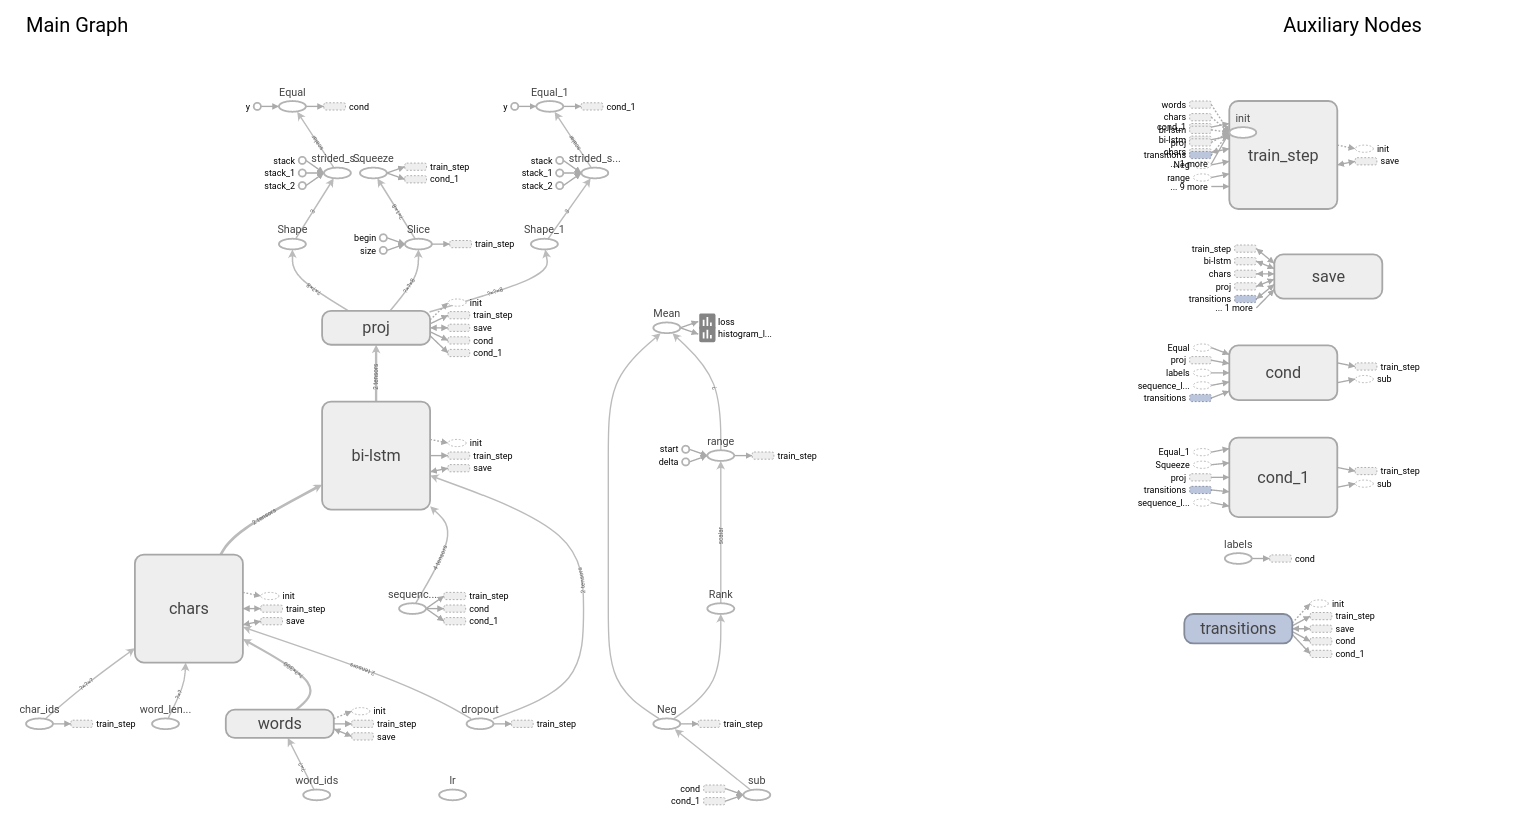
\includegraphics[width=6.5in]{images/finalGraph.png}
  \caption {Final graph}
  \label{fig:finalGraph}
\end{figure}

We now have the built-in network, now it has to be trained and tested.

\begin{lstlisting}[language=Python,caption={Train network}]
    def train(self, train: CoNLLDataset, dev: CoNLLDataset):
        best_score = 0
        n_epoch_no_improve = 0  # for early stopping
    
        for epoch in range(self.config.n_epochs):
            score = self._run_epoch(train, dev, epoch)
            self.config.lr *= self.config.lr_decay  # decay learning rate
    
            if score >= best_score:
                n_epoch_no_improve = 0
                best_score = score
                self.save_session()
            else:
                n_epoch_no_improve += 1
                if n_epoch_no_improve >= self.config.n_epoch_no_improve:
                    break
    
    def _run_epoch(self, train: CoNLLDataset, dev: CoNLLDataset, epoch) -> int:
        n_batches = (len(train) + self.config.batch_size - 1) // self.config.batch_size

        # iterate over dataset
        for i, (words, labels) in enumerate(minibatches(train, self.config.batch_size)):
            fd, _ = self.get_feed_dict(words, labels, self.config.lr, self.config.dropout)

            _, train_loss, summary = self.sess.run([self.train_op, self.loss, self.merged], feed_dict=fd)

        metrics = self._run_evaluate(dev)

        return metrics["f1"]
\end{lstlisting}

As mentioned above, the network will be fed with a small number of sentences of the same length. So for that we need a tool that uniformises sentences and characteristics too. In other words, to transforms the words in there ids based on the dictionary and bring them in the same form.

\begin{lstlisting}[language=Python,caption={Make embeddings}]
    def pad_sequences(sequences, sequences_length=None):
        sequences_length = max(
            map(lambda x: len(x) if type(x) is not int else 0, sequences)) if sequences_length is None else sequences_length
    
        seqs = []
        lengths = []
        for sequence in sequences:
    
            seq = fill_array(sequence if type(sequence) is not int else [sequence], sequences_length)
            length = len(sequence) if type(sequence) is not int else 0
    
            if type(sequence) is not int and type(sequence[0]) == list:
                max_length_word = max([max(map(lambda x: len(x), _seq)) for _seq in sequences])
    
                # seq = list(map(lambda x: [x] if type(x) == int else x, seq))
                seq, length = pad_sequences(seq, max_length_word)
    
            lengths += [length]
            seqs += [seq]
    
        return seqs, lengths
\end{lstlisting}

Now we can feed the network. For that need to fit placeholders dimensions.

\begin{itemize}
    \item word\_ids: (batch size, max length of sentence in batch)
    \item sequence\_lengths: (batch size)
    \item char\_ids: (batch size, max length of sentence in batch, max length of word in sentence)
    \item word\_lengths: (batch size, max length of sentence in batch)
    \item labels: (batch size, max length of sentence in batch)
\end{itemize}

\begin{lstlisting}[language=Python,caption={Feed network}]
    def get_feed_dict(self, words, labels=None, lr=None, dropout=None):

        char_ids, word_ids = zip(*words)

        word_ids, sequence_lengths = pad_sequences(word_ids)
        char_ids, word_lengths = pad_sequences(char_ids)

        # build feed dictionary
        feed = {
            self.word_ids: word_ids,
            self.sequence_lengths: sequence_lengths,
            self.char_ids: char_ids,
            self.word_lengths: word_lengths
        }

        if labels is not None:
            labels, _ = pad_sequences(labels)
            feed[self.labels] = labels

        if lr is not None:
            feed[self.lr] = lr

        if dropout is not None:
            feed[self.dropout] = dropout

        return feed, sequence_lengths
\end{lstlisting}

There are two types of evaluation for neural network, one based on exact match (f1) and index matching.

In statistical analysis of binary classification, the F1 score (also F-score or F-measure) is a measure of a test's accuracy. It considers both the precision p and the recall r of the test to compute the score: p is the number of correct positive results divided by the number of all positive results returned by the classifier, and r is the number of correct positive results divided by the number of all relevant samples (all samples that should have been identified as positive). The F1 score is the harmonic average of the precision and recall, where an F1 score reaches its best value at 1 (perfect precision and recall) and worst at 0.

\begin{equation*}
     F_1=2 * \frac {precision * recall} {precision + recall}
\end{equation*}

\begin{lstlisting}[language=Python,caption={Test network}]
    def _run_evaluate(self, test: CoNLLDataset):
        accs = []
        correct_preds, total_correct, total_preds = 0., 0., 0.
        for words, labels in minibatches(test, self.config.batch_size):
            labels_pred, sequence_lengths = self.predict_batch(words)

            for lab, lab_pred, length in zip(labels, labels_pred,
                                             sequence_lengths):
                lab      = lab[:length]
                lab_pred = lab_pred[:length]
                accs    += [a==b for (a, b) in zip(lab, lab_pred)]

                cond = lambda x: x[0] != self.config.vocab_tags[NONE]   

                lab_chunks = set(filter(cond, get_chunks(lab, self.config.vocab_tags)))
                lab_pred_chunks = set(filter(cond, get_chunks(lab_pred, self.config.vocab_tags)))

                correct_preds += len(lab_chunks & lab_pred_chunks)
                total_preds += len(lab_pred_chunks)
                total_correct += len(lab_chunks)

        p = correct_preds / total_preds if correct_preds > 0 else 0
        r = correct_preds / total_correct if correct_preds > 0 else 0
        f1 = 2 * p * r / (p + r) if correct_preds > 0 else 0
        acc = np.mean(accs)

        return {"acc": 100 * acc, "f1": 100 * f1}

    def predict_batch(self, words):

        fd, sequence_lengths = self.get_feed_dict(words, dropout=1.0)

        viterbi_sequences = []
        logits, trans_params = self.sess.run([self.logits, self.trans_params], feed_dict=fd)

        for logit, sequence_length in zip(logits, sequence_lengths):
            logit = logit[:sequence_length] 
            viterbi_seq, viterbi_score = tf.contrib.crf.viterbi_decode(logit, trans_params)
            viterbi_sequences += [viterbi_seq]

        return viterbi_sequences, sequence_lengths
\end{lstlisting}

\subsubsection{Tests}

Reteteau has been tested on several types of configurations. The best results were obtained with the following configurations.

\begin{lstlisting}[language=Python,caption={Network configurations}]
    n_epochs = 5
    dropout = 0.5  # rate to randomize
    batch_size = 20  # nb of sentence
    lr_method = "adam"
    lr = 0.001  # learn rate
    lr_decay = 0.9  # adjust learn rete
    n_epoch_no_improve = 3

    hidden_size_char_lstm = 100  # lstm on chars
    hidden_size_word_lstm = 300  # lstm on word embeddings
\end{lstlisting}

It is to be noted that the training of the network takes about 25 minutes with these configurations.

\begin{lstlisting}[language=Python,caption={Network results during training}]
    2018-04-15 00:31:01,504 - logger - INFO - Initializing tf session
    2018-04-15 00:31:02,658 - logger - INFO - Epoch 1 out of 5
    2018-04-15 00:36:10,565 - logger - INFO - acc 97.13 - f1 81.56
    2018-04-15 00:36:10,990 - logger - INFO - - new best score!
    2018-04-15 00:36:10,990 - logger - INFO - Epoch 2 out of 5
    2018-04-15 00:41:07,991 - logger - INFO - acc 97.67 - f1 86.18
    2018-04-15 00:41:08,586 - logger - INFO - - new best score!
    2018-04-15 00:41:08,586 - logger - INFO - Epoch 3 out of 5
    2018-04-15 00:46:02,616 - logger - INFO - acc 97.97 - f1 88.25
    2018-04-15 00:46:03,339 - logger - INFO - - new best score!
    2018-04-15 00:46:03,339 - logger - INFO - Epoch 4 out of 5
    2018-04-15 00:50:58,869 - logger - INFO - acc 98.18 - f1 89.35
    2018-04-15 00:50:59,477 - logger - INFO - - new best score!
    2018-04-15 00:50:59,477 - logger - INFO - Epoch 5 out of 5
    2018-04-15 00:55:53,944 - logger - INFO - acc 98.22 - f1 89.87
    2018-04-15 00:55:54,455 - logger - INFO - - new best score!
\end{lstlisting}

One of the results obtained after training is the following
\begin{equation*}
    acc = 97.21;
    f1 = 85.23;
\end{equation*}


\begin{figure}[H]
  \centering
  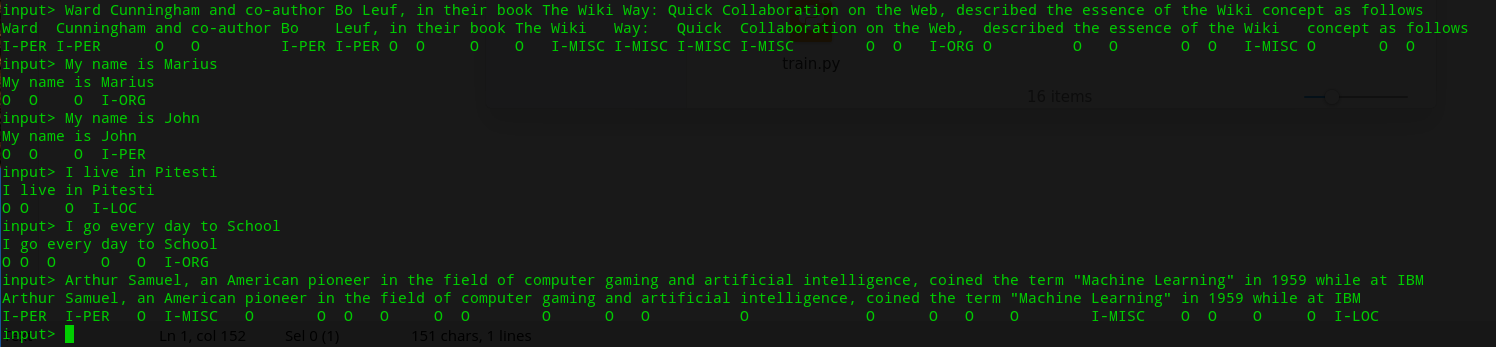
\includegraphics[width=6.5in]{images/interactive.png}
  \caption {Some of the interactive results}
\end{figure}

Here's how the loss diagram shows:

\begin{figure}[H]
  \centering
  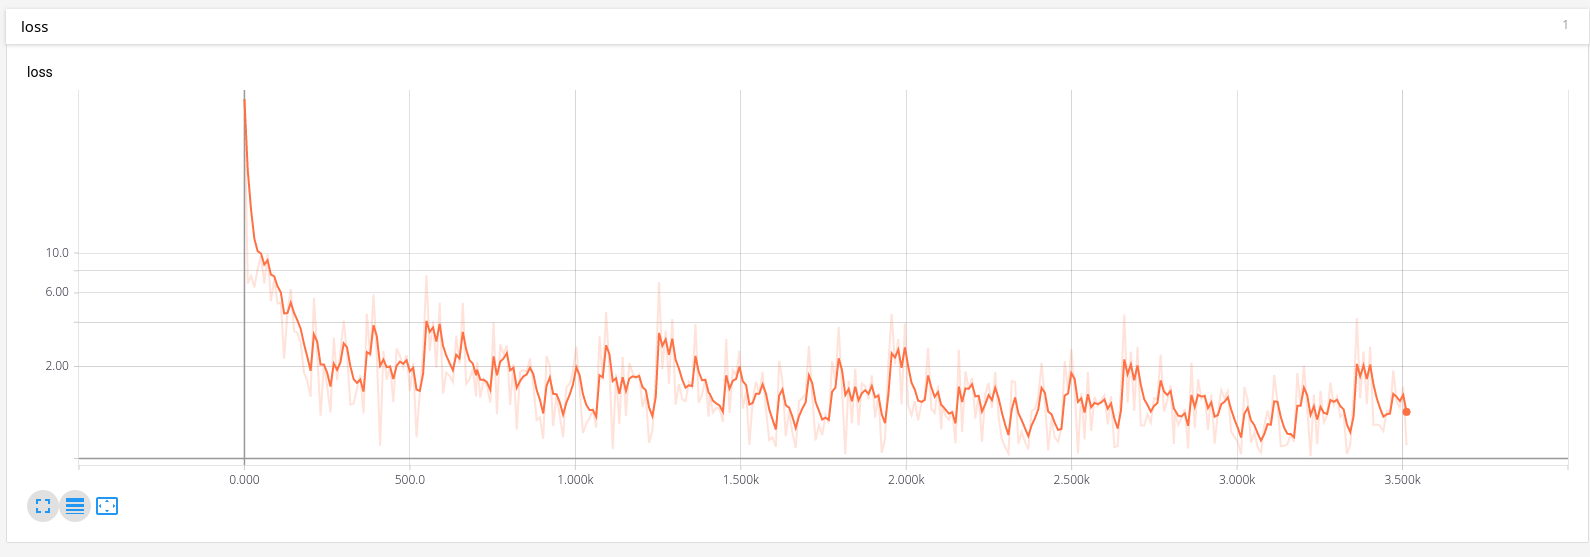
\includegraphics[width=6.5in]{images/loss.png}
  \caption {Loss diagram}
\end{figure}

Tensor board also provides a way of representing words. You can also see the links between Gloved words.

\begin{figure}[H]
  \centering
  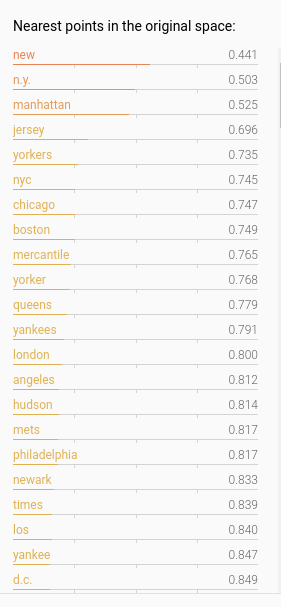
\includegraphics[width=2.5in]{images/york.png}
  \caption {Distance for word "York"}
\end{figure}
